% homework
% 20161121
% by hiaoxui

\documentclass[a4paper, 12pt, notitlepage]{article}

\usepackage{CJKutf8}
\usepackage{indentfirst}
\usepackage{amsmath}
\usepackage{listings}
\usepackage{longtable}
\usepackage{graphicx}
\usepackage{float}

\setlength{\parindent}{2em} 

\begin{CJK*}{UTF8}{gbsn}
\begin{document}

\title{第八次OS作业}
\author{秦光辉\ 1500011398}
\maketitle

\section{系统调用实现过程}

	实际上系统调用语句本身是硬件提供的(机器指令), 但其所调用的功能是操作系统提供的. 每种机器的机器指令集中都有一条系统调用指令. \\
	
\begin{enumerate}
	\item 设置系统调用号和参数. 调用号作为指令的一部分或者装入到特殊的寄存器里. 参数装入特殊的寄存器, 或者寄存器指针指向参数表. 
	\item 执行trap(int)指令. 入口的一般性处理, 查入口跳转表, 跳转到相应功能的过程. 保护CPU现场(将PC与PSW入栈),改变CPU执行状态(处理机状态字PSW切换,地址空间表切换). 同时将参数取到核心空间.
	\item 执行操作系统内部代码. 
	\item 执行iret指令: 将执行结果装入适当位置(类似于参数带入), 恢复CPU现场(以栈顶内容置PSW和PC).
\end{enumerate}

\section{ }

	有5个批处理的作业(a, b, c, d, e)几乎同时到达一个计算中心, 估计运行时间分别为2, 4, 6, 8, 10分钟, 它们的优先数分别为1, 2, 3, 4, 5(1为最低优先级). 对下面的每种调度算法, 分别写出作业运行顺序, 并计算作业的平均周转时间和平均带权周转时间

\subsection{最高优先级优先}

\begin{align*}
	T &= \frac{10 + 18 + 24 + 28 + 30}{5} = 22 \\
	W &= \frac{10/10 + 18/8 + 24/6 + 28/4 + 30/2}{5} = 5.85
\end{align*}

\subsection{FCFS}

\begin{align*}
	T &= \frac{6 + 14 + 18 + 28 + 30}{5} = 19.2 \\
	W &= \frac{6/6 + 14/8 + 18/4 + 28/10 + 30/2}{5} = 5.01
\end{align*}

\subsection{SJF}

\begin{align*}
	T &= \frac{2 + 6 + 12 + 20 + 30}{5} = 14 \\
	W &= \frac{2/2 + 6/4 + 12/6 + 20/8 + 30/10}{5} = 2
\end{align*}

\section{ }

	有一个具有两道作业的批处理系统,作业调度采用短作业优先的调度算法,进程调度采用以优先数为基础的抢占式调度算法,有如表所示的作业序列(表中所列的作业优先数即为进程优先数,数值越小优先级越高). \\
	
\subsection{列出所有作业进入内存时间及结束时间}

	10点A进入系统, 被作业调度装入系统, 被内存调度调度, 开始运行. \\
	
	10点20, B作业被作业调度装入系统, 被内存调度调度, A被就绪, B开始运行. \\
	
	10点30, C作业等待被调度. \\
	
	10点50, B作业完成, 退出系统. 同时D也开始等待被调度. 由于D运行时间较短, 进入系统. A继续运行. \\
	
	11点10分, A运行结束, C作业被作业调度调度, 进入内存. C开始被运行. \\
	
	12点, C运行结束, 退出. D开始被运行. \\
	
	12点20, D运行结束, 退出.

\subsection{计算平均周转时间}

\begin{align*}
	T = \frac{70 + 30 + 90 + 90}{4} = 70
\end{align*}

\section{银行家算法问题}

\subsection{该状态是否安全}

	给P0分配资源, 回收, 剩余资源数为1 6 5 4. \\
	
	给P3分配资源, 回收, 剩余资源数为1 9 8 6. \\
	
	给P1分配资源, 回收, 剩余资源数为2 9 8 6. \\
	
	给P4分配资源, 回收, 剩余资源数为2 9 9 10. \\
	
	给P2分配资源, 回收, 剩余资源数为3 12 14 14. \\
	
	该状态是安全的!

\subsection{若进程P2提出请求request(1, 2, 2, 2)后, 系统能否将资源分配给它}

	给P2分配1 2 2 2, 剩余资源数为0 4 0 0. \\
	
	0 4 0 0无法满足任何进程的要求, 所以系统不安全, 所以系统不能将资源分配给P2.

\section{ }

	一个操作系统有20个进程, 竞争使用65个同类资源, 申请方式是逐个进行的, 一旦某进程获得它所需要的全部数量, 立即归还所有资源. 每个进程最多使用3个资源. 若仅考虑这类资源, 该系统有无可能全部死锁, 为什么? \\
	
	答: 一共有20个进程, 每个进程需要3个以下的资源, 所需资源数最多为60个, 但是剩余资源数大于60, 故不可能死锁!
	
\section{ }

	假定某计算机系统有R1和R2两类可再使用资源(其中R1由两个单位, R2有一个单位), 它们被进程P1和P2所共享, 且已知两个进程均以申请R1$->$申请R2$->$申请R1$->$释放R1$->$释放R2$->$释放R1$->$所示的顺序使用两类资源.

\subsection{试求出系统运行过程中可能达到的死锁点}

	一个简单的死锁点就是, 进程P1申请R1, 申请R2之后, 进程P2申请R1, 等待申请R2. 此时P1无法申请到R1从而无法继续进行, P2无法申请到R2从而也无法继续进行, 进入死锁状态.

\subsection{画出死锁点的资源分配图}

\begin{figure}[h]
\centering
	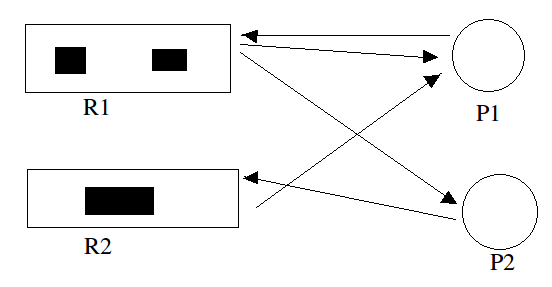
\includegraphics[scale=0.7]{hw8_figure.png}
\end{figure}

\end{CJK*}
\end{document}